\chapter{Evaluation \label{evaluation}}
The implementation of the modified client and the controller was tested using mininet. The evaluation focuses on the modified client and the controller which are the results of this thesis. The software for the switch was written by M.Apostolaki from ETH Zürich.\\
The evaluation starts with a general setup in \ref{evaluation:setup}. This shows that the protocol is working as expected. Additionally, we measure the speed of the block distribution. After analysing the scaling properties of the protocol in section \ref{evaluation:scaling} and comparing the message sizes of the proposed solution to the state-of-the-art bitcoin client in \ref{evaluation:messages}, we measure the memory and CPU overhead in sections \ref{evaluation:memory} and \ref{evaluation:cpu} respectively.

\begin{figure}[!hbt]
  \begin{center}
	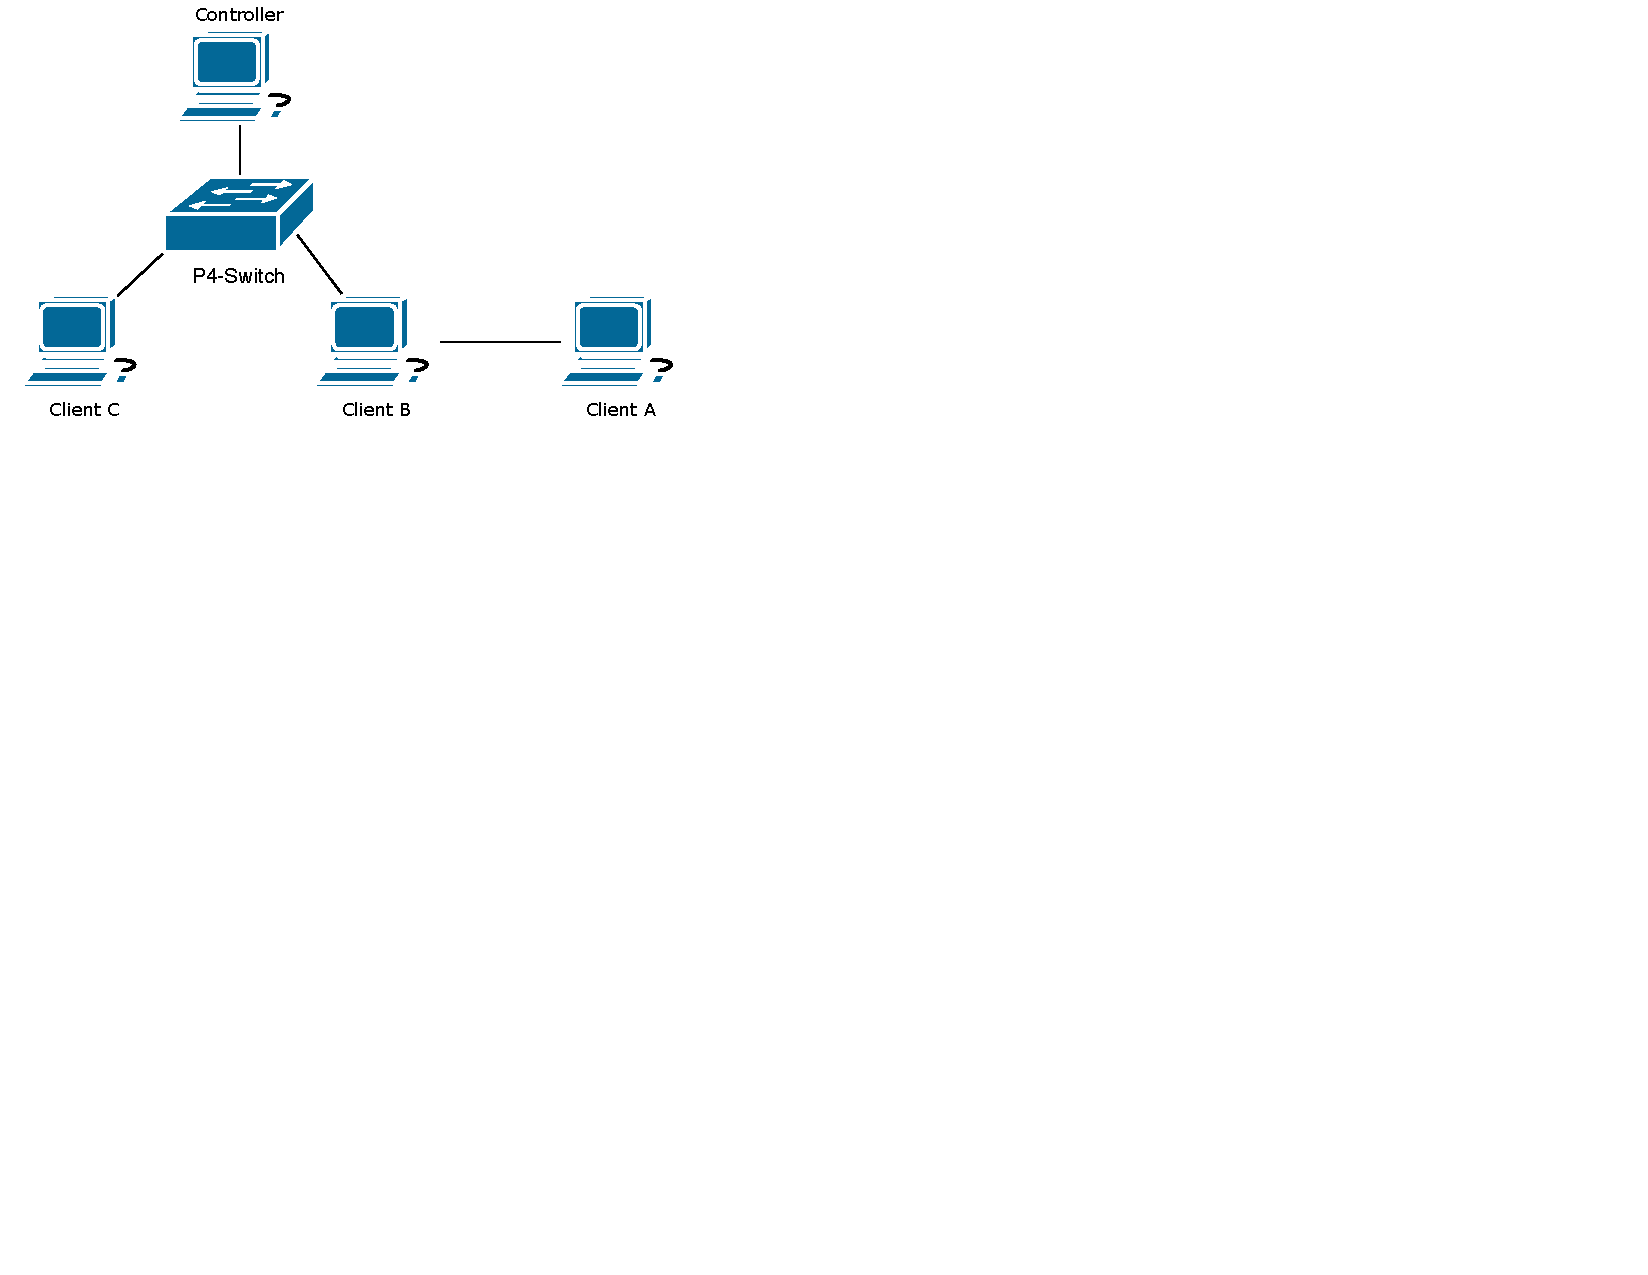
\includegraphics[width=0.5\textwidth]{Figures/Test_setup.pdf}
	  \end{center}

  \caption[Overview of the test setup used for the evaluation.]{Overview of the test setup used for the evaluation. Client A is a \textit{regular bitcoin client} that has 1 block that clients B/C and the\textit{controller} do not posses. Clients B and C are \textit{modified bitcoin clients}. The switch is a programmable P4-switch emulated in software.}
  \label{figure:test_setup}
\end{figure}

\section{\label{evaluation:setup}Functional evaluation}
Using mininet, a small test setup was created. The setup consists of 3 clients, one switch and a controller. An overview of the setup can be seen in figure \ref{figure:test_setup}. Client A is a \textit{regular bitcoin client} and clients B and C are \textit{modified bitcoin clients}. The controller is a bitcoin relay \textit{controller} as described in section \ref{design:SwitchController}. The test covers 2 important use cases. First, it shows that the \textit{modified client} is able to interact with the \textit{regular bitcoin client} and that therefore an incremental deployment in the bitcoin network is possible. Second, the update and advertisement process described in the \textit{relay protocol} is tested. 
\subsubsection{Setup}
The experiment goes through the following steps.
\begin{enumerate}
	\item Client A has a block that the other clients and the controller do not yet have in their local storage.
	\item Clients B and C do a handshake with the switch.
	\item Client A establishes a connection to client B.
	\item Client A advertises its latest block to client B using the regular bitcoin network protocol.
	\item Upon receiving the block, client B advertises the block to the switch.
	\item The switch does not know the block and sends a CTR message to client B indicating that it should connect to the controller.
	\item Client B establishes a connection to the controller.
	\item Client B sends its latest block to the controller using the regular bitcoin network protocol.
	\item The controller updates the switch and advertises the new block to all clients.
	\item Client C does not have the block in its local storage and requests the block from the switch and adds it to its chain.
\end{enumerate}
Note that there is no direct connection between clients B and C. To make sure that clients A and B establish a connection, the IP of client A was whitelisted at client B.\\
This setting was run with 10 different blocks and was repeated 20 times for each block which results in a total of 200 experiment runs. The mean block size was 1128194 bytes during the experiment. This means that there are 2261 segments in average.\\
\subsubsection{Results}
After each run, the log files that are generated by the clients and the controller are analysed. From this data, we can calculate the time needed for the block to travel from node B through the controller and the switch to client C.\\
We are interested in the time client B needs to connect to the controller. For this, we measure the time between the moment when client B adds a new block to the chain until the moment when the connection between the client and the controller is established. We see that after 2ms, the client sends an ADV message and receives a CON response from the switch 2ms later. The client then needs 11ms to connect to the controller. So in total, the client is connected 15ms after it received the block. After connecting, the client and the controller need 4.7s to transfer the new block from the client to the controller.\\
At the controller, we want to measure the time needed to update the switch. For this we measure the time starting from the moment when the controller adds the new block to its chain until the last BLK message is sent. We focus on the work done at the controller and neglect the time of flight of the packet and the overhead at the switch. We measure an update time of 3.4s. Remember that a 1ms delay was introduced when sending the block segments. With 2261 segments this means that there is a 2.26s delay which explains a part of the overhead. 7ms after the last segment is sent, the RINV message to the client is sent.\\
Lastly, we want to see how fast client C can request the block from the switch. For this, we measure the time between the moment when client C receives the RINV message and the moment when the block is added to the chain. We see, that the last segment of the block arrives after 4.3s. Again, the 2.26 seconds of transmission delay has to be taken into account here. After that, 3.9s is needed to verify the block and add it to the chain. The overhead here stems from the fact that the client has to verify all transactions that are contained in the block because they were not previously available to the client. In total, the block request takes 8.3s from the moment the RINV message is received. This is 52\% slower than the transmission of the block from client B to the controller that was using the regular bitcoin protocol. 
The whole process, starting from the moment client B receives the block until client C receives it takes 16.3s. To speed up this process, one could first investigate, if the 1ms delay is needed in actual hardware. This would reduce the measured time by 4.5s. Further, a future adaption could allow storing of transactions at the switch which would reduce the time needed by client C to add the new block to its chain. However, most of the time overhead can be regarded as setup cost for the cache at the switch. A more realistic scenario would be, when there is not a single client C but many clients that are interested in the block and are able to request it in parallel.

% this is new
%t1=0.002152884665367122
%t2=0.004278595191682911
%t3=0.014793193372319689
%t4=4.667016932781028
%t5=8.025114057147498
%t6=8.032396441975308
%t7=8.033542145451593
%t8=12.373263397368422
%t9=16.311130394704353
%size=1128193.6666666667


\section{Scaling \label{evaluation:scaling}}
To inspect the scaling behaviour of the controller, a python based pseudo client is crated which will open 1'000 connections to the relay. The test setup is the same as in section \ref{evaluation:setup}, but with client C replaced by 1'000 clients. After the pseudo client has set up the connections, it waits for incoming RINV messages and logs the arrival time of the last incoming RINV message. We run the test with 3 different blocks and 3 runs each. The time needed to send the 1'000 RINV messages is 1.24s. There is a 1ms delay between each message which accounts for 1s of the time needed. If the delay can be removed when working with real hardware, the 1'000 RINV messages are expected to be sent out in 240ms. As we expect the switch to be able to process requests at line rate, we do not expect a large overhead for the clients to request the blocks from the switch. However, this claim could not be verified with the software emulated switch.\\
Next, the connection count is further increased and the system stats are measured. We use the same setup as in sections \ref{sec:perf_degen} and \ref{sec:generalResources} but use the relay controller. The measurement is made on \textit{device 1}. We let the setup connect to 30 regular nodes  and use a python client to add 10'000 relay connections by sending emulated CON messages. The rest of the test setup is equal to the one defined in the before mentioned sections. CPU, I/O, Swap and Memory measurements show no significant overhead over the setup without the 10'000 relay connections. The results of the measurement can be seen in table \ref{tab:evaluation:generalresources}. The measurement of the RTT shows 19'335$\mu s$, which is comparable to about 200-300 regular connections according to table \ref{tab:performance_degeneration}. The measured delay can be explained by the overhead that is generated, when a new block arrives. If we assume a block that is split into 2500 segments, there are 12'500 messages (INV and BLK) that are sent per block. As there is an artificial delay of 1ms after every message, this means that there is a 12.5s overhead for each block. We assume to be able to greatly reduce the overhead when using a hardware switch.







\begin{table}[tbp]
\begin{center}	
\begin{tabular}{l|l|l|r }
\textbf{category} & \textbf{Parameter} & \textbf{Unit} & \textbf{30} \\
\hline
CPU & User & \%             & 1.36 \\
    & Sys  & \%             & 0.79  \\
    & Idle & \%             & 97.43 \\
    & Context switches & /5s  & 1'454.08 \\
\hline
I/O & Interrupts & /5s       & 673.37 \\
    & Disk reads   & /5s     & 150.35 \\
    & Disk writes   & /5s    & 26.87 \\
    & I/O wait     & s/5s       & 0.48 \\
\hline
Swap & Swap   & KB          & 7.21 \\
\hline
Memory & Free memory  & KB          & 114'138 \\
       & used Buffer space  & KB    & 67'954.4 \\
\end{tabular}
\caption[General resource measurements of the modified bitcoin client.]{General resource usage measurement on \textit{device 1} when connected to 10'000 nodes via the relay.}
\label{tab:evaluation:generalresources}
\end{center}
\end{table}











\section{Bandwidth overhead\label{evaluation:messages}}
The current bitcoin protocol specifies different ways to transmit blocks from one client to another. Most of the optimisations aim at smaller block messages to be able to speed up the block distribution. The optimisations relay on prefetching transactions so that the client is able to pre-verify the transactions. This makes it difficult to compare the message of the relay transmitted block size to the one needed by the current bitcoin protocol. Instead, we calculate the overhead compared to a traditional block message.
\subsubsection{Client}
First, we focus on the overhead introduced by the protocol. The relay message protocol specifies a payload size of 499 bytes. If we define $s_i$ as the size of the block message (block + header) and $s_r$ as the total cumulated message size of all segments, we can express $s_r$ by adding the overhead of the new header per segment and the padding overhead to $s_i$
\begin{equation}
	s_r = s_i+ \left\lceil \frac{s_i}{499B} \right\rceil \cdot 5B + s_i \mbox{ mod } 499
\end{equation}
Currently, blocks have the size of about 1MB. If we assume $504B \ll s_i$, we can express the protocol overhead as  
\begin{equation} \label{eq:overhead}
	\frac{s_r}{s_i} \approx 1+\frac{5}{499} = 1.01
\end{equation}
The 499 maximum payload size is smaller than the most commonly used MTU of TCP. This means, that the transport layer also adds an overhead to the transmitted block size. We assume a commonly used MTU of 1500 bytes for the calculations. Further we assume 24 bytes Ethernet headers, 20 bytes IP headers, 20 bytes TCP headers and 8 bytes UDP headers. We denote the transmitted message size of the regular and the relay blocks as $t_i$ and $t_r$ respectively. We get the following expressions
\begin{equation}
	t_i = s_i + \left\lceil \frac{s_i}{1500} \right\rceil(24 + 20 + 20)B
\end{equation} 
\begin{equation}
	t_r = s_r + \left\lceil \frac{s_r}{499} \right\rceil(24 + 20 + 8)B
\end{equation} 
Assuming $1500B \ll s_i$ and $499B \ll s_r$, we can estimate the bandwidth overhead as
\begin{equation} \label{eq:throughput}
	\frac{t_r}{t_i}\approx \frac{s_r}{s_i} \cdot\frac{1+\frac{52}{499}}{1+\frac{64}{1500}} = 1.07
\end{equation}
This rough estimate shows that we can expect overhead of about 7\% when comparing to a minimal TCP based transmission. The overhead could be reduced if the protocol would be changed to support larger payloads than 499 bytes. However, as the discovery of a new block is a sporadic event, this should not pose a large drawback.\\
So far, only the bandwidth overhead of incoming messages were observed. As each segment of the block has to be requested, the protocol also generates overhead on the outgoing messages. We compare the total amount of outgoing messages to a single getdata message of the regular bitcoin protocol. Getdata was chosen over other block exchange mechanisms such as headers messages, because getdata has the smallest foodprint. This will give us an estimate on the upper bound on the overhead. The getdata message with a single block hash has a size of 61 bytes. Per 499 bytes of block, the modified client has to send a request of size 37 bytes. On the other hand, the regular client sends TCP ACKs. If we assume a block of size 1MB, a TCP MTU of 1500B, 24B ethernet headers, 20B IP headers and 8B UDP headers and assume a lossless transmission, we get the following overhead:
\begin{equation}
	\frac{\left\lceil \frac{1MB}{499B} \right\rceil \cdot (37B + 52B)}{61B + 64B + \left\lceil \frac{1MB}{1500B} \right\rceil\cdot 64B} = 4.2
\end{equation}
In other words, the request size is increased by the factor 4.2 when comparing the relay protocol to the regular bitcoin protocol. This is limited by the protocol and can only be changed when changing the protocol or when increasing the data chunk size of the segments. However, as the requests of the individual segments is pipelined, this does not lead to a large overhead time wise. 



\subsubsection{Controller}
To send blocks, the controller has to update the switch. Similarly to equations \ref{eq:overhead} and \ref{eq:throughput}, the overhead can be calculated. Here, we have to add the overhead from the UPD message (35 bytes) and the additional checksum in the headers of the BLK messages (+2 bytes). However, as we have $35B \ll s_i$ and $\frac{5}{499}\approx\frac{7}{499}$, we get
\begin{equation}
	\frac{s_r}{s_i} \approx 1+\frac{7}{499} = 1.014
\end{equation}
and 
\begin{equation} \label{eq:throughput}
	\frac{t_r}{t_i}\approx \frac{s_r}{s_i} \cdot\frac{1+\frac{52}{499}}{1+\frac{64}{1500}} = 1.074
\end{equation}
for the outgoing message overhead.\\
The update process has to be done once per block. Except from the single 37 byte INV message per client, there is no additional overhead when the block is sent to multiple clients. This is a clear benefit when compared to the regular client, which needs to send the block for each peer that requests it.





















\section{Memory overhead \label{evaluation:memory}}
Let's first inspect the memory usage of the controller.
Let $m_0$ be the amount of memory needed to store the state of a single peer-to-peer connection. Let $m_b^n$ and $m_r^n$ be the amount of memory needed to store the state of n peer-to-peer connections and n relay connections, respectively. To maintain the basic connection to the relay, we use the same data structure as used by peer-to-peer connections. The connection uses a UDP connection instead of a TCP connection which uses less state, therefore we can say that
\begin{equation}
	m_r^0 \leq m_b^1 = m_0
\end{equation}
When adding new connections, a new data structure is added for the regular connections. For the relay connections, the metadata of the the peer is stored in the existing data structure. This leads to the following overhead
\begin{equation}
	m_b^n = n\cdot m_0
\end{equation}
\begin{equation}
	m_r^n = m_0 + n\cdot 6B
\end{equation}
While the actual size of the data structure can vary across compilers and operating systems, with gcc 5.4.0 on Ubuntu 16.04.1 we have $m_0 = 1672B$. This means that we use less than 1\% of the size of regular connections for the relay connections.\\
On the client, the connection to the switch uses the same data structure as regular connections. This means, that the memory usage is the same in user space. In kernel space, the memory overhead is smaller, because the UDP connection that is used needs to store less state.







\section{CPU overhead\label{evaluation:cpu}}
To measure the CPU overhead of the design, we use the same test setup as in section \ref{sec:workAnalysis}. We let the node establish 30 connections and add 10'000 relay connections using a pseudo client which emulates the CON messages from the switch before starting the profiler. Again, we let the experiment run for 4h and repeat it 3 times. The addition to the system accounts for 3.1\% of the total CPU time of the MessageHandler thread. From the results we can see that there is no significant overhead in adding 10'000 relay connections.





\section{Conclusion}
With this evaluation, we show that the presented solution has better scalability characteristics than the state-of-the-art bitcoin client. It was shown that the controller can handle multiple thousands of connections with a minimal memory and CPU overhead. The tradeoff for this increased scalability is the increased bandwidth needed by the clients and the slower block propagation. We expect to greatly improve the block propagation speed when running with a hardware switch instead of an emulated one.




















